\subsection{Blazemark}
Blazemark is a benchmark suite provided by Blaze to compare the performance of Blaze with other linear algebra libraries including Blitz++\cite{Blitz}, Boost uBLAS\cite{Boost}, GMM++\cite{GMM++}, Armadillo\cite{sanderson2016armadillo}, MTL4\cite{MTL}, and Eigen3\cite{Eigen}, alongside plain BLAS libraries like Atlas\cite{ATLAS}, Goto\cite{gotoblas}, and Intel MKL.\cite{MKL}

\begin{figure}[H]
	\centering
	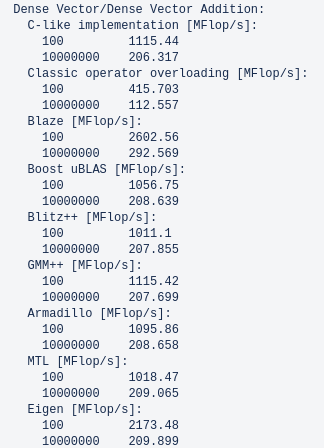
\includegraphics[scale=0.5]{images/blazemark_1.png}
	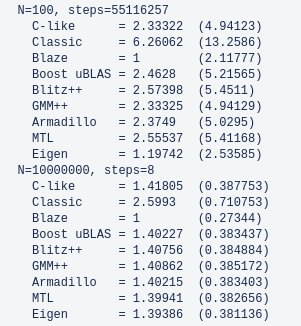
\includegraphics[scale=0.5]{images/blazemark_2.png}
	\caption{An example of the results obtained from running $DVECDVECADD$ benchmark through Blazemark}	
	\label{blazemark1}
\end{figure}


\vspace{\baselineskip}	
\section{Parallelization in Blaze}
Depending on the operation and the size of operands, this assignment could be parallelized through four different backends, namely, HPX, OpenMP\cite{dagum1998openmp}, C++ threads, and Boost\cite{Boost}. 
Table~\ref{table2} shows the default value for some of the threshold for parallelization applied to operations performed in Blaze. It should be noted that these thresholds should be tuned based on the parallelization backend and also the system architecture.
%For matrix matrix multiplication alongside the mentioned thresholds, there exists another set of thresholds to switch between using Blaze kernels or BLAS kernels. 
%As stated in Section~\ref{Background} Blaze being based on smart expression templates, offers the option to use either Blaze or a highly optimized kernel for computations. This option is set at compile time through $BLAS_mode$ macro. If $BLAS_mode=1$, 

\vspace{\baselineskip}	
\begin{table}[H]
	\centering
	\resizebox{\textwidth}{!}
	{\begin{tabular}{|c | c |} 
			\hline
			Benchmark & Array size \\ [0.5ex] 
			\hline
			\hline
			$DVECDVCEADD$, $DVECDVECMULT$ & 38000\\ 	
			\hline
			$DMATDMATADD$ & 36100 elements equivalent to a $175\times{175}$ matrix \\
			\hline	
			$DMATDMATMULT$ & 3025 elements equivalent to a $55\times{55}$ matrix  \\
			\hline			
	\end{tabular}}
	
	\caption{List of some of the thresholds applied to the operations performed by Blaze, starting from which the operation is executed in parallel}
	\label{table2}
\end{table} 

\vspace{\baselineskip}	
\subsection{Implementation of HPX Backend}
As stated earlier, as an ET-based library, blaze performs the calculations when an expression is assigned to a target, which is implemented through the \textit{blaze::Assign} function.

The four mentioned backends, parallelize this assignment process through a parallel for-loop, in which at each iteration a specific section of each of the vectors or matrices(called a block) is selected and assigned to a core. Each core then performs the operation on the block they have been assigned to.  

Each backend uses their own method for parallelizing this for loop. For HPX backend, current implementation uses a HPX \textit{parallel::for\textunderscore loop} with static chunking policy and chunk size of 1. This way, knowing the number of cores to run the application on, we can divide the original matrix equally among the cores, while the order of assignment of blocks to the cores is known at compile time.  
Listings\ref{old_hpx_backend} shows the current implementation of the HPX backend in Blaze.

\begin{lstlisting}[float,floatplacement=H,caption= {Previous implementation of Assign function for HPX backend in Blaze.}, label={old_hpx_backend}]
template< typename MT1   // Type of the left-hand side dense matrix
, bool SO1       // Storage order of the left-hand side dense matrix
, typename MT2   // Type of the right-hand side dense matrix
, bool SO2       // Storage order of the right-hand side dense matrix
, typename OP >  // Type of the assignment operation
void hpxAssign( DenseMatrix<MT1,SO1>& lhs, const DenseMatrix<MT2,SO2>& rhs, OP op )
{
using hpx::parallel::for_loop;
using hpx::parallel::execution::par;

BLAZE_FUNCTION_TRACE;

using ET1 = ElementType_t<MT1>;
using ET2 = ElementType_t<MT2>;

constexpr bool simdEnabled( MT1::simdEnabled && MT2::simdEnabled && IsSIMDCombinable_v<ET1,ET2> );
constexpr size_t SIMDSIZE( SIMDTrait< ElementType_t<MT1> >::size );

const bool lhsAligned( (~lhs).isAligned() );
const bool rhsAligned( (~rhs).isAligned() );

const size_t threads    ( getNumThreads() );
const ThreadMapping threadmap( createThreadMapping( threads, ~rhs ) );

const size_t addon1     ( ( ( (~rhs).rows() % threadmap.first ) != 0UL )? 1UL : 0UL );
const size_t equalShare1( (~rhs).rows() / threadmap.first + addon1 );
const size_t rest1      ( equalShare1 & ( SIMDSIZE - 1UL ) );
const size_t rowsPerThread( ( simdEnabled && rest1 )?( equalShare1 - rest1 + SIMDSIZE ):( equalShare1 ) );

const size_t addon2     ( ( ( (~rhs).columns() % threadmap.second ) != 0UL )? 1UL : 0UL );
const size_t equalShare2( (~rhs).columns() / threadmap.second + addon2 );
const size_t rest2      ( equalShare2 & ( SIMDSIZE - 1UL ) );
const size_t colsPerThread( ( simdEnabled && rest2 )?( equalShare2 - rest2 + SIMDSIZE ):( equalShare2 ) );

for_loop( par, size_t(0), threads, [&](int i)
{
const size_t row   ( ( i / threadmap.second ) * rowsPerThread );
const size_t column( ( i % threadmap.second ) * colsPerThread );

if( row >= (~rhs).rows() || column >= (~rhs).columns() )
return;

const size_t m( min( rowsPerThread, (~rhs).rows()    - row    ) );
const size_t n( min( colsPerThread, (~rhs).columns() - column ) );

if( simdEnabled && lhsAligned && rhsAligned ) {
auto       target( submatrix<aligned>( ~lhs, row, column, m, n ) );
const auto source( submatrix<aligned>( ~rhs, row, column, m, n ) );
op( target, source );
}
else if( simdEnabled && lhsAligned ) {
auto       target( submatrix<aligned>( ~lhs, row, column, m, n ) );
const auto source( submatrix<unaligned>( ~rhs, row, column, m, n ) );
op( target, source );
}
else if( simdEnabled && rhsAligned ) {
auto       target( submatrix<unaligned>( ~lhs, row, column, m, n ) );
const auto source( submatrix<aligned>( ~rhs, row, column, m, n ) );
op( target, source );
}
else {
auto       target( submatrix<unaligned>( ~lhs, row, column, m, n ) );
const auto source( submatrix<unaligned>( ~rhs, row, column, m, n ) );
op( target, source );
}
} );
}
\end{lstlisting}

What we suggest here is that, some prior knowledge for example, architecture of the system we are running the application on, the expression that has to be executed, number of cores of the system, size and type of the arrays we are dealing with, and etc. should be able to help us to achieve a higher performance.
For this purpose we introduced two parameters block\textunderscore{size} and chunk\textunderscore{size}.

\begin{lstlisting}[float,floatplacement=H,caption= {New implementation of Assign function for HPX backend in Blaze.}, label={new_hpx_backend}]
template< typename MT1   // Type of the left-hand side dense matrix
, bool SO1       // Storage order of the left-hand side dense matrix
, typename MT2   // Type of the right-hand side dense matrix
, bool SO2       // Storage order of the right-hand side dense matrix
, typename OP >  // Type of the assignment operation
void hpxAssign( DenseMatrix<MT1,SO1>& lhs, const DenseMatrix<MT2,SO2>& rhs, OP op )
{
using hpx::parallel::for_loop;
using hpx::parallel::execution::par;

BLAZE_FUNCTION_TRACE;

using ET1 = ElementType_t<MT1>;
using ET2 = ElementType_t<MT2>;

constexpr bool simdEnabled( MT1::simdEnabled && MT2::simdEnabled && IsSIMDCombinable_v<ET1,ET2> );
constexpr size_t SIMDSIZE( SIMDTrait< ElementType_t<MT1> >::size );

const bool lhsAligned( (~lhs).isAligned() );
const bool rhsAligned( (~rhs).isAligned() );

const size_t threads    ( getNumThreads() );
const size_t numRows ( min( static_cast<std::size_t>( BLAZE_HPX_MATRIX_BLOCK_SIZE_ROW ), (~rhs).rows() ) );
const size_t numCols ( min( static_cast<std::size_t>( BLAZE_HPX_MATRIX_BLOCK_SIZE_COLUMN ), (~rhs).columns() ) );

const size_t rest1      ( numRows & ( SIMDSIZE - 1UL ) );
const size_t rowsPerIter( ( simdEnabled && rest1 )?( numRows - rest1 + SIMDSIZE ):( numRows ) );
const size_t addon1     ( ( ( (~rhs).rows() % rowsPerIter ) != 0UL )? 1UL : 0UL );
const size_t equalShare1( (~rhs).rows() / rowsPerIter + addon1 );

const size_t rest2      ( numCols & ( SIMDSIZE - 1UL ) );
const size_t colsPerIter( ( simdEnabled && rest2 )?( numCols - rest2 + SIMDSIZE ):( numCols ) );
const size_t addon2     ( ( ( (~rhs).columns() % colsPerIter ) != 0UL )? 1UL : 0UL );
const size_t equalShare2( (~rhs).columns() / colsPerIter + addon2 );

hpx::parallel::execution::dynamic_chunk_size chunkSize ( BLAZE_HPX_MATRIX_CHUNK_SIZE );

for_loop( par.with( chunkSize ), size_t(0), equalShare1 * equalShare2, [&](int i)
{
const size_t row   ( ( i / equalShare2 ) * rowsPerIter );
const size_t column( ( i % equalShare2 ) * colsPerIter );

if( row >= (~rhs).rows() || column >= (~rhs).columns() )
return;

const size_t m( min( rowsPerIter, (~rhs).rows()    - row    ) );
const size_t n( min( colsPerIter, (~rhs).columns() - column ) );

if( simdEnabled && lhsAligned && rhsAligned ) {
auto       target( submatrix<aligned>( ~lhs, row, column, m, n ) );
const auto source( submatrix<aligned>( ~rhs, row, column, m, n ) );
op( target, source );
}
else if( simdEnabled && lhsAligned ) {
auto       target( submatrix<aligned>( ~lhs, row, column, m, n ) );
const auto source( submatrix<unaligned>( ~rhs, row, column, m, n ) );
op( target, source );
}
else if( simdEnabled && rhsAligned ) {
auto       target( submatrix<unaligned>( ~lhs, row, column, m, n ) );
const auto source( submatrix<aligned>( ~rhs, row, column, m, n ) );
op( target, source );
}
else {
auto       target( submatrix<unaligned>( ~lhs, row, column, m, n ) );
const auto source( submatrix<unaligned>( ~rhs, row, column, m, n ) );
op( target, source );
}
} );
}
\end{lstlisting}
\vspace{\baselineskip}	
\subsection{HPX \textit{for\textunderscore loop}}
HPX \textit{for\textunderscore loop} takes an execution policy as first argument, which is set to \textit{dynamic\textunderscore chunk\textunderscore size} execution policy in case of HPX backend for Blaze.

\vspace{\baselineskip}	
\section{Experiments}
In order to capture the relationship between number of cores, \textit{chunk\textunderscore{size}}, \textit{block\textunderscore{size}}, and the performance, we ran a series of experiments with different of these parameters and measured the number of floating point operations per second performed. 

For these experiments ,at the first step we selected the $DMatDMatADD$ benchmark which was implemented in Blazemark. $DMatDMatADD$ benchmark is a level 3 BLAS function to perform matrix-matrix addition in the form of $A=B+C$, where $A$, $B$, $C$ are square matrices of the same size. 

To avoid adding the scheduling overhead for small matrix sizes, Blaze uses a threshold to start parallelization, which is specific to the type of operation. For matrix-matrix addition, if the number of elements in the matrix is greater than 36100 elements(which is equivalent to a square matrix of size 190$\times$190) Blaze uses the configured backend to parallelize the assignment operation. For this reason, we start our experiments with matrix size of 200x200 and gradually increase the size to 1587$\times$1587. 
Table~\ref{table1} show the matrix sizes and the number of cores chosen for our experiments with $DMATDMATADD$ benchmark.

\vspace{\baselineskip}	
\begin{table}[H]
	\centering
		\resizebox{\textwidth}{!}
		{\begin{tabular}{|c | c |} 
			\hline
			Matrix sizes & 200, 230, 264, 300, 396, 455, 523, 600, 690, 793, 912, 1048, 1200, 1380, 1587 \\ [0.5ex] 
			\hline
			Number of cores & 1, 2, 3, 4, 5, 6, 7, 8 \\ 	
			\hline
			Number of rows in the block & 4, 8, 12, 16, 20, 32 \\
			\hline	
			Number of columns in the block & 64, 128, 256, 512, 1024 \\
			\hline
			Chunk size & Between 1 and total number of blocks (logarithmic increase)\\\hline
		\end{tabular}}

		\caption{List of different values used for each variable for running the $DMATDMATADD$ benchmark}
		\label{table1}
\end{table}




Figure~\ref{fig1} shows the results of running $DMatDMatADD$ benchmark for matrix sizes and number of cores listed in \tablename{name} based on grain size. 

On the other hand, Figure~\ref{fig4} integrates the results obtained from running the same benchmark with different matrix sizes. Each color in this graph represents a specific matrix size. 

\begin{figure}[H]
	\centering
	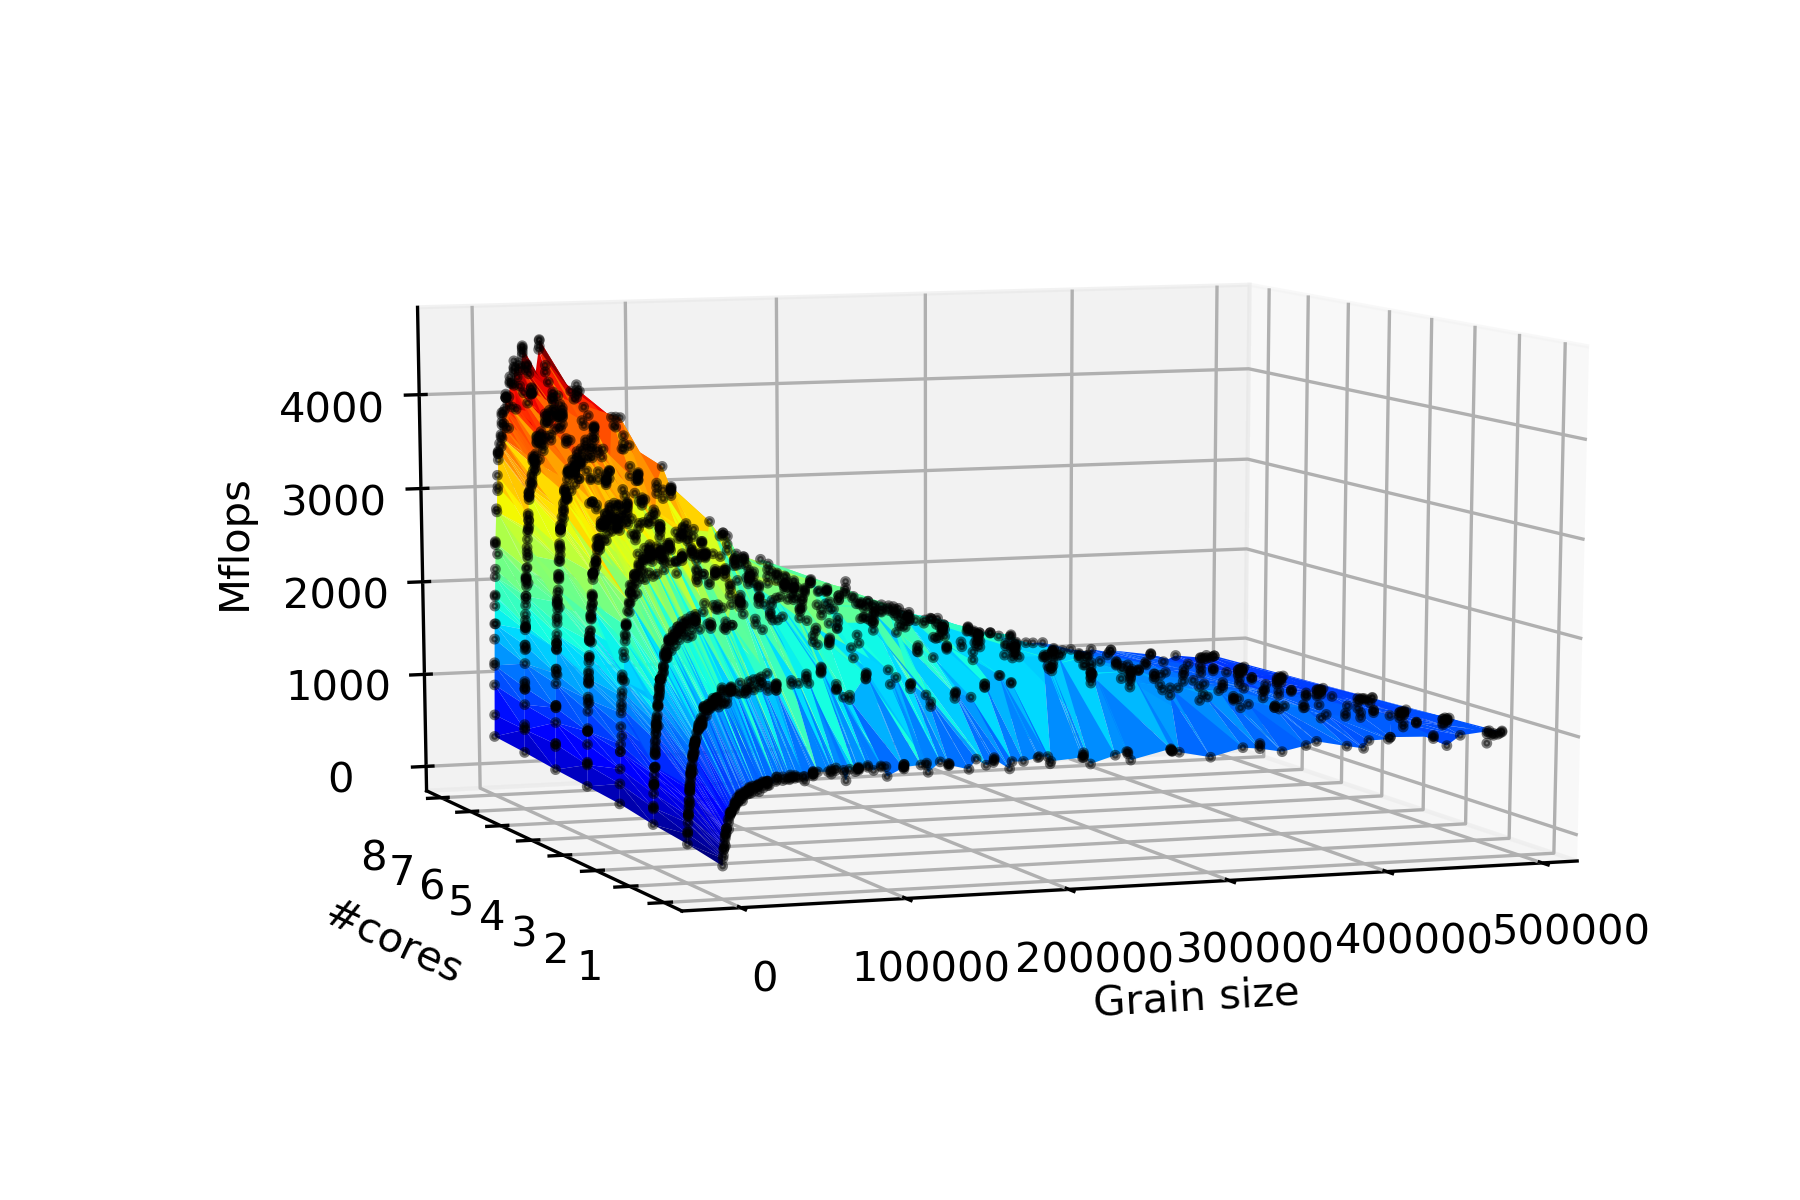
\includegraphics[width=1\linewidth]{images/fig2.png}
	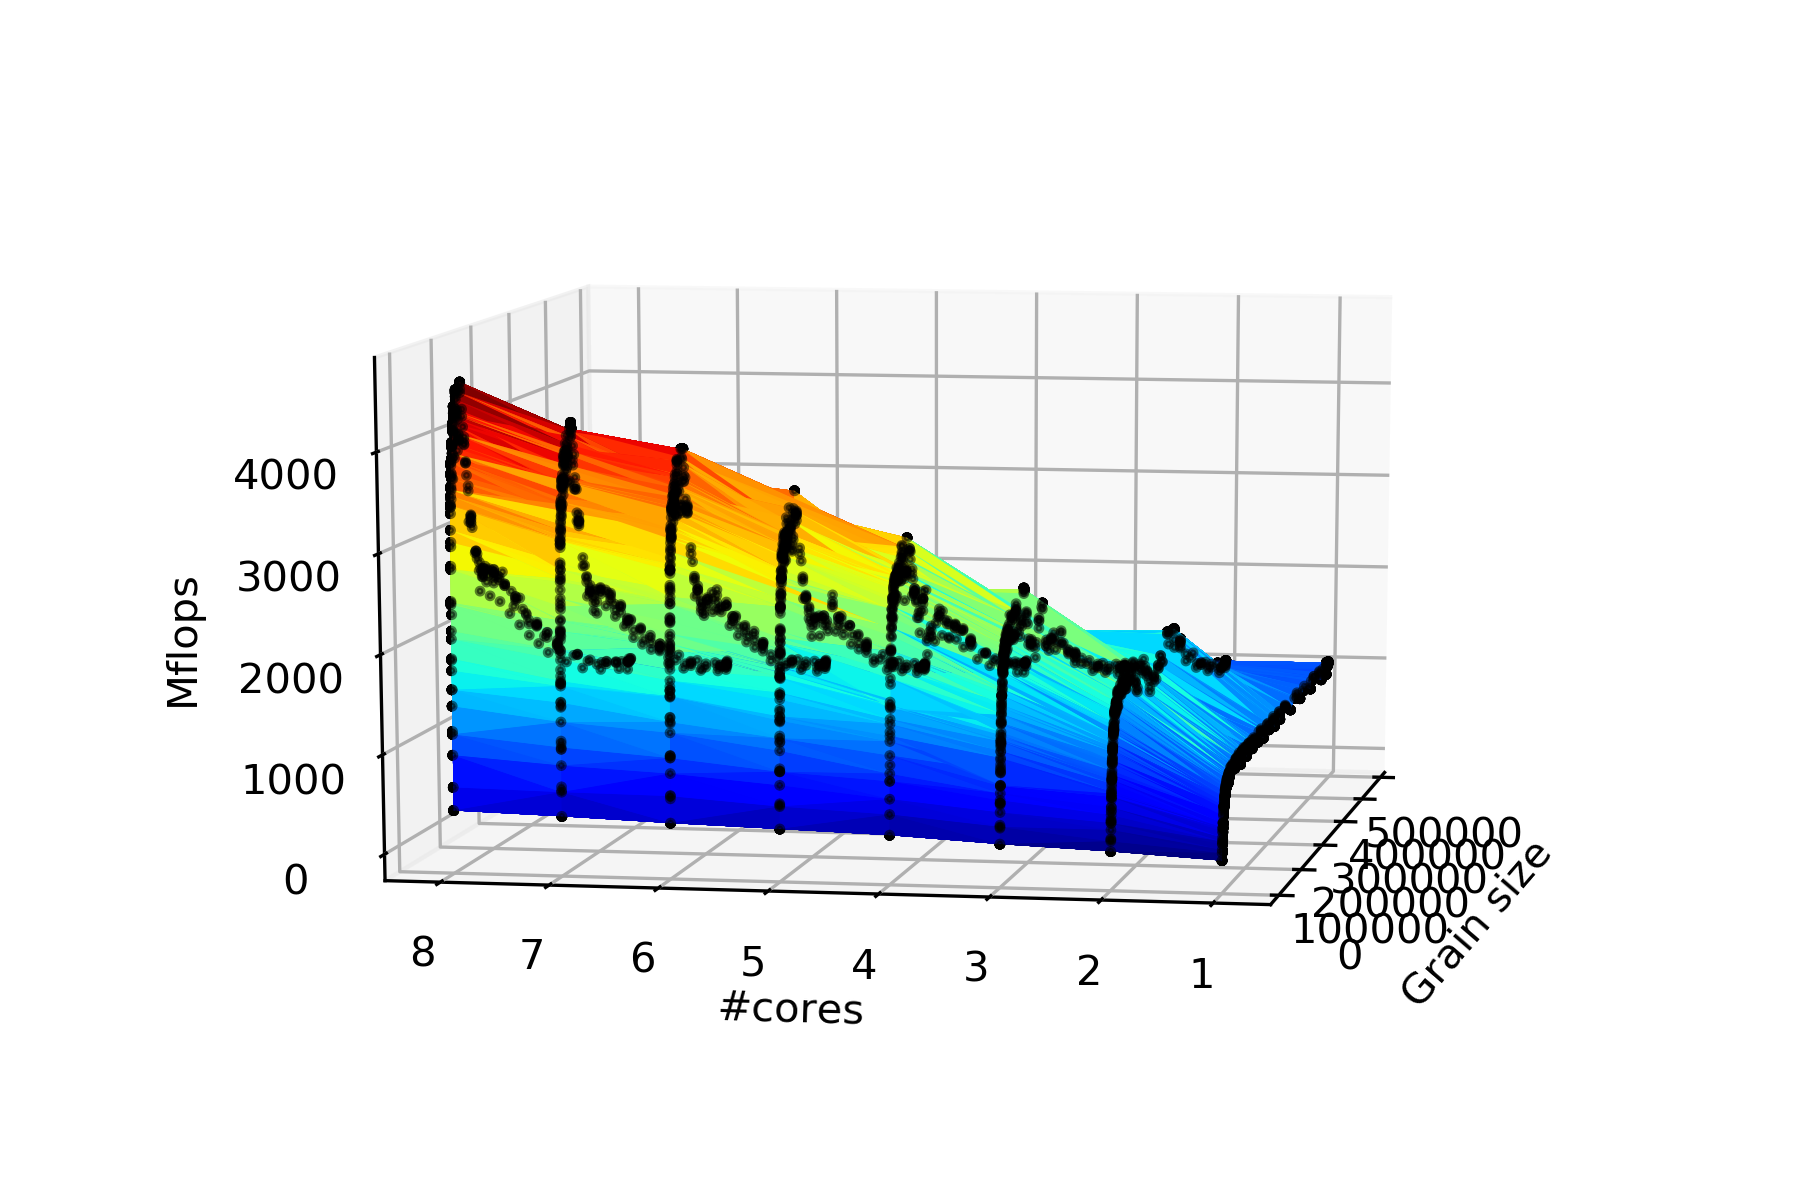
\includegraphics[width=1\linewidth]{images/fig3.png}
	\caption{The results obtained from running $DMATDMATADD$ benchmark through Blazemark for matrix of size 690$\times$690 from two different angles}	
	\label{fig1}
\end{figure}

\begin{figure}[H]
	\centering
	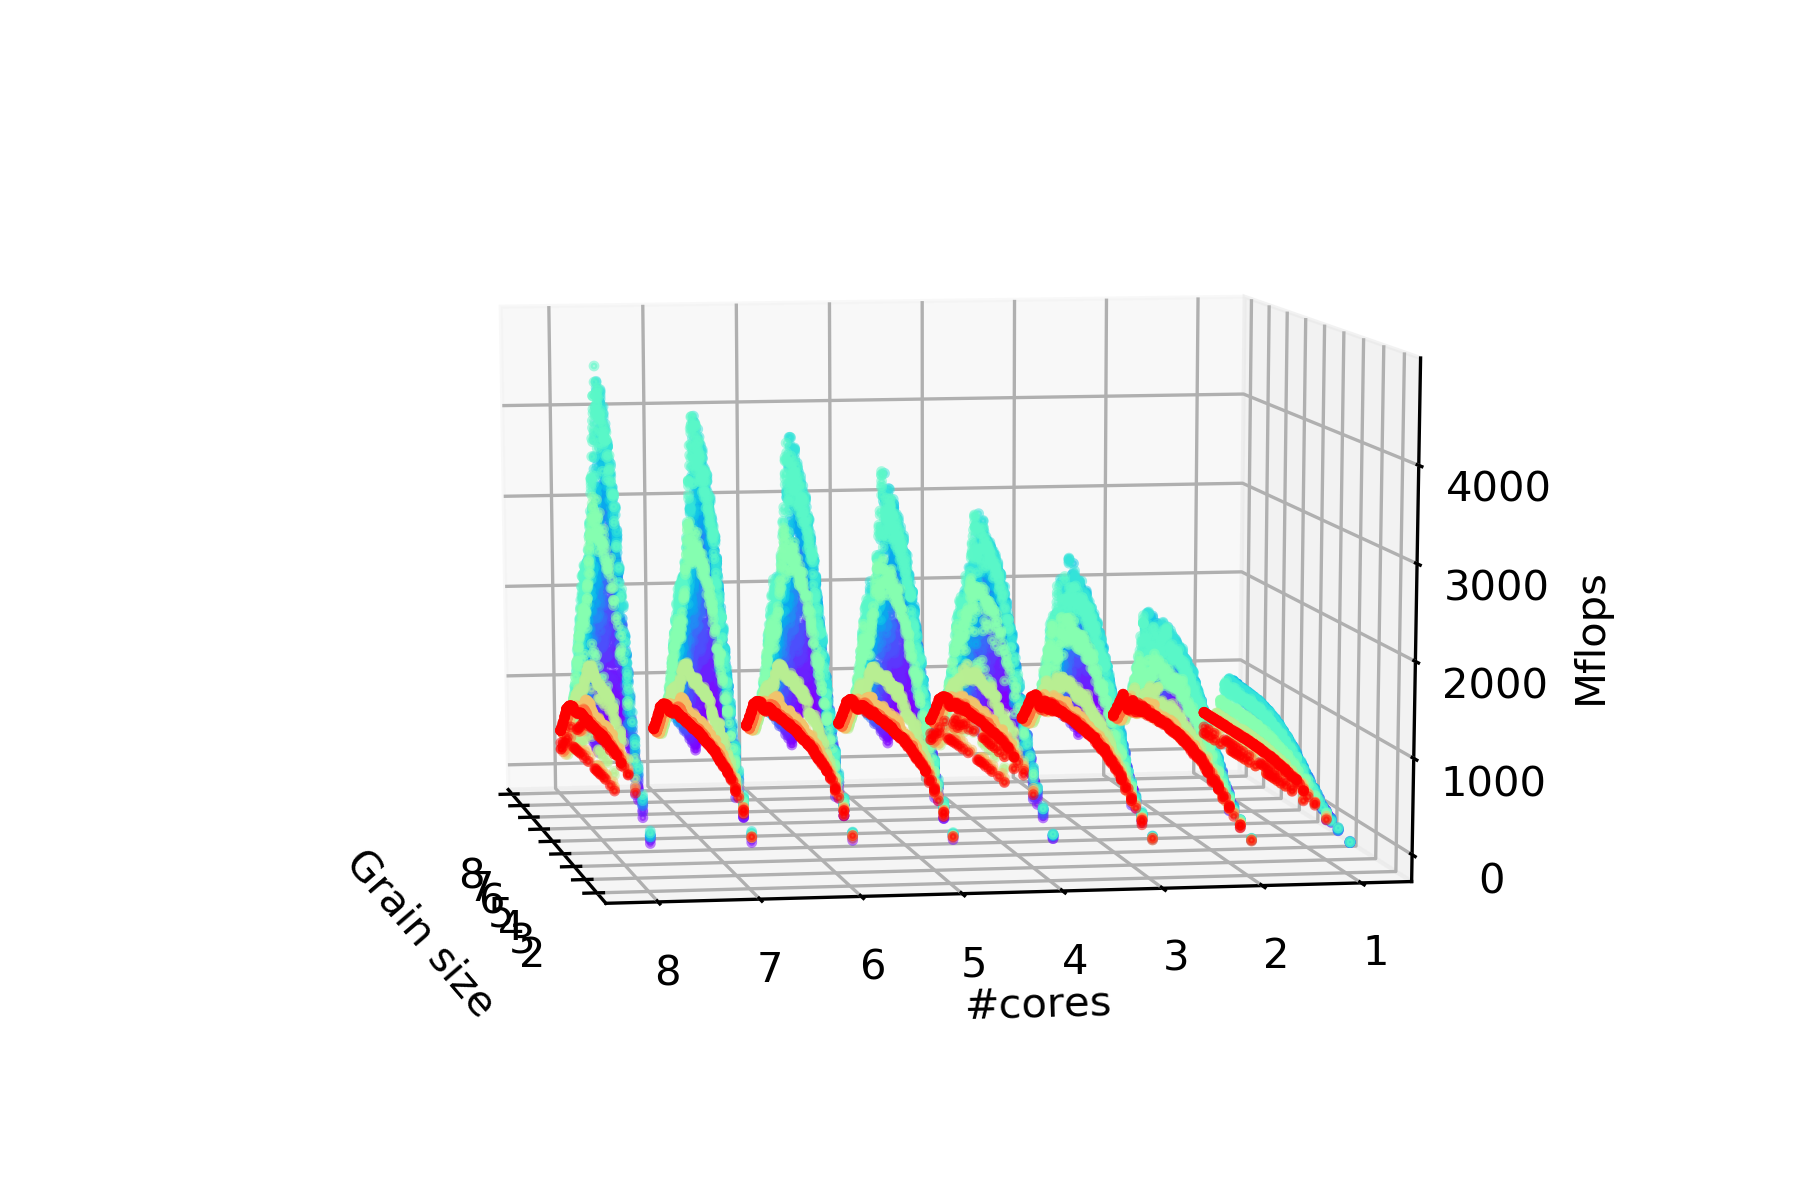
\includegraphics[width=1\linewidth]{images/fig4.png}
	\caption{The results obtained from running $DMATDMATADD$ benchmark through Blazemark for matrix sizes from 200$\times$200 to 1587$\times$1587}	
	\label{fig4}
\end{figure}


\subsection{Observation}
The final purpose of our experiments is to find a chunk size that gives us the best performance for a given matrix size on a given machine. This chunk size should also be tailored to the expression being executed, and this all is based on assuming that we have already fixed the block size.
So the first step appeared to be selecting the block size. For this purpose, we ran the experiments with a selection of block sizes as shown in Table~\ref{table1}.


It should be mentioned that there were three constraints on selecting the block sizes. First, Blaze forces the number of columns in a raw-major matrix to be divisible to SIMD register size in order to be able to take advantage of vectorization. Second, we have selected the number of columns in our blocks to be either divisible by cache line or to contain all the columns of the matrix.     


\begin{figure}[H]
	\centering
	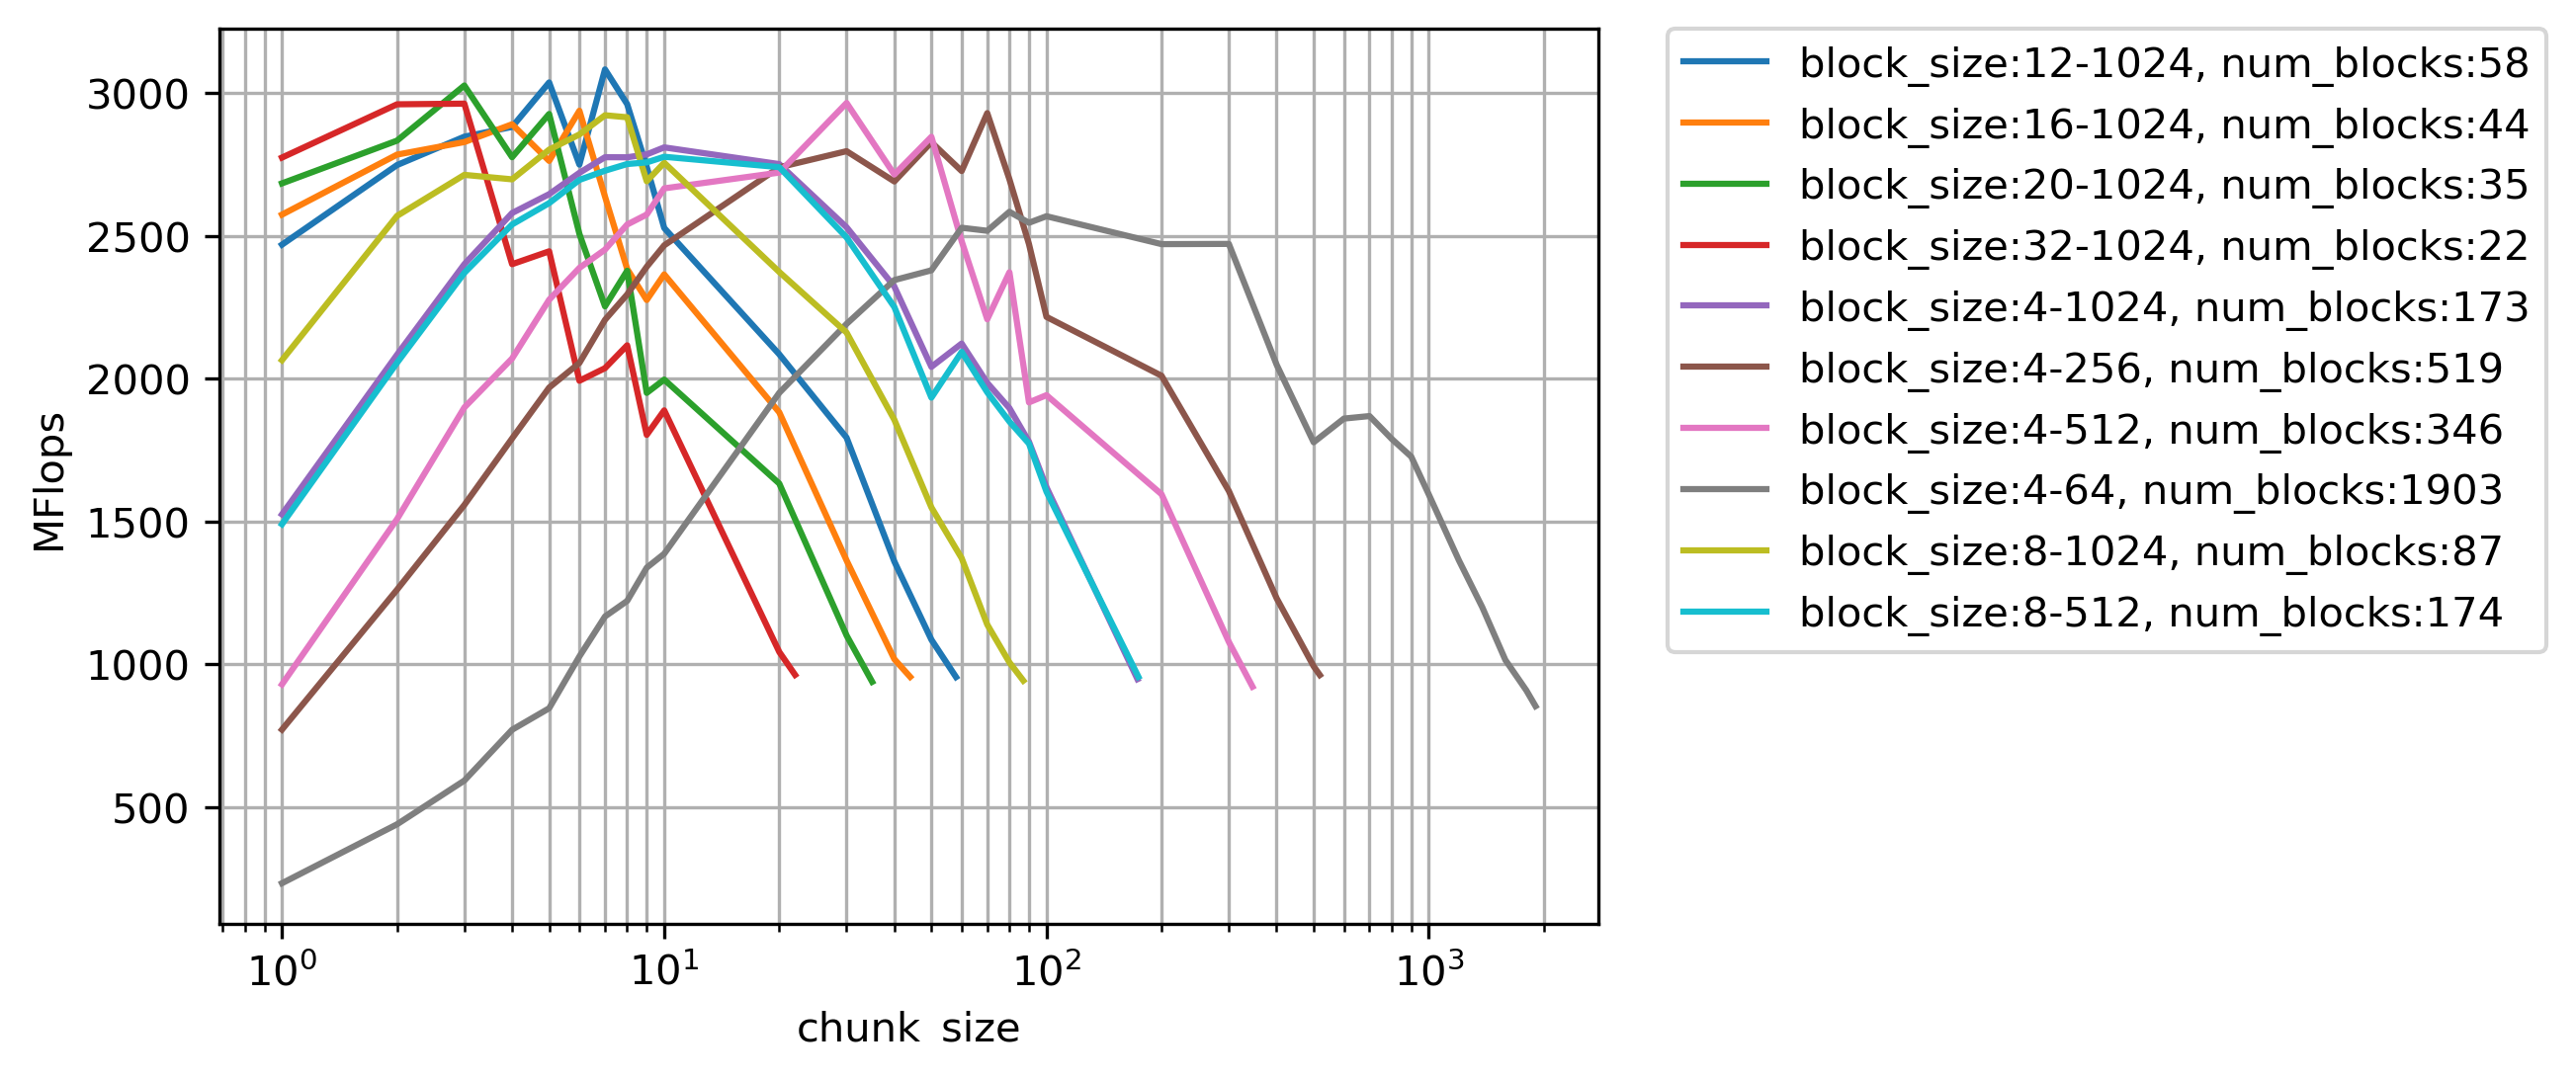
\includegraphics[width=1\linewidth]{images/fig5.png}
	\caption{The results obtained from running $DMATDMATADD$ benchmark through Blazemark for matrix sizes from 690$\times$690 with different combinations of block size and chunk size on $4$ cores}	
	\label{fig5}
\end{figure}

The collected data, as seen in Figure~\ref{fig5}, suggests two main points:
\begin{itemize}
	\item For each selected block size, there is a range of chunk sizes that gives us the best performance. 
	\item Except for some uncommon cases, no matter which block size we choose, we are able to achieve the maximum performance if we select the right chunk size.  
\end{itemize}

This motivated us to move our search parameter from chunk size to grain size. As stated earlier, grain size is the amount of work assigned to one HPX thread. Here we represent grain size by number of floating point operations performed by a HPX thread. For example, performing addition among two matrices, if we choose the block size as $4\times64$ and chunk size as $3$, the grain size would be $3\times4\times64=768$. 
Note that in our experiments whenever the number of columns of the original matrix is not divisible to the selected number of columns for block size, there would be a set of blocks with less number of elements than the selected block size, this has been considered when calculating the grain size.  

By changing our focus to the grain size instead of the block size and the chunk size, Figure~\ref{fig6} shows how the throughput changes with regards to the grain size for the $DMATDMATADD$ benchmark, for each specific block size. Each combination of block size and chunk size generates a point in the graph. On the other hand, Figure~\ref{fig9} looks at these graphs from another aspect, keeping the problem size constant but changing the number of the cores to run the benchmark on, instead.

\begin{figure}[H]
	\centering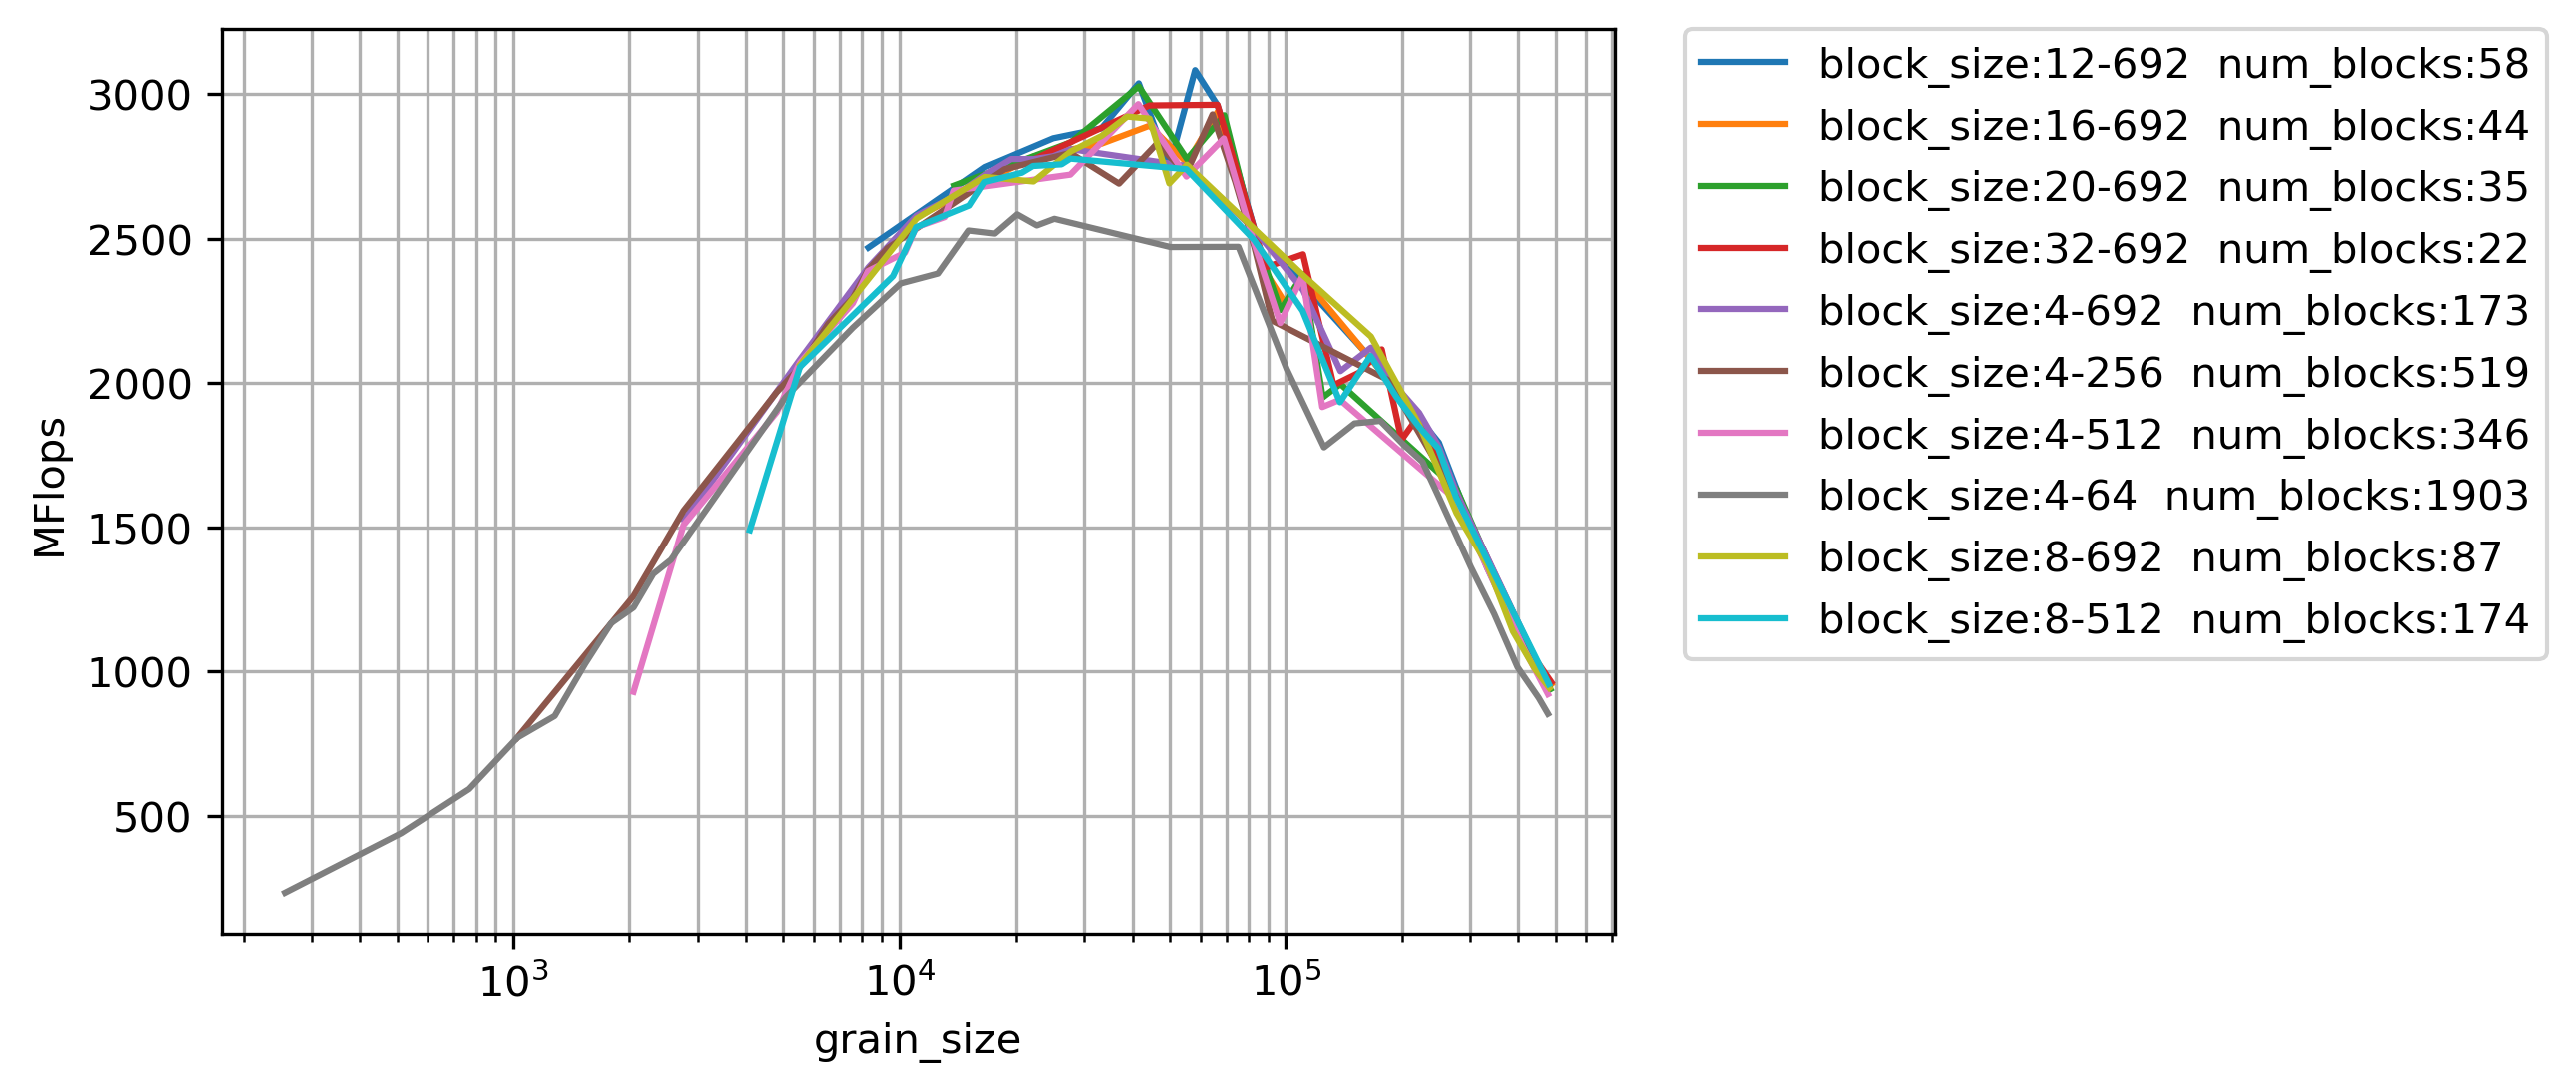
\includegraphics[width=1\linewidth]{images/fig6.png}
	\caption{The results obtained from running $DMATDMATADD$ benchmark through Blazemark for matrix size 690$\times$690 on $4$ cores}	
	\label{fig6}
\end{figure}

\begin{figure}[H]
	\centering
	\hspace*{-2cm}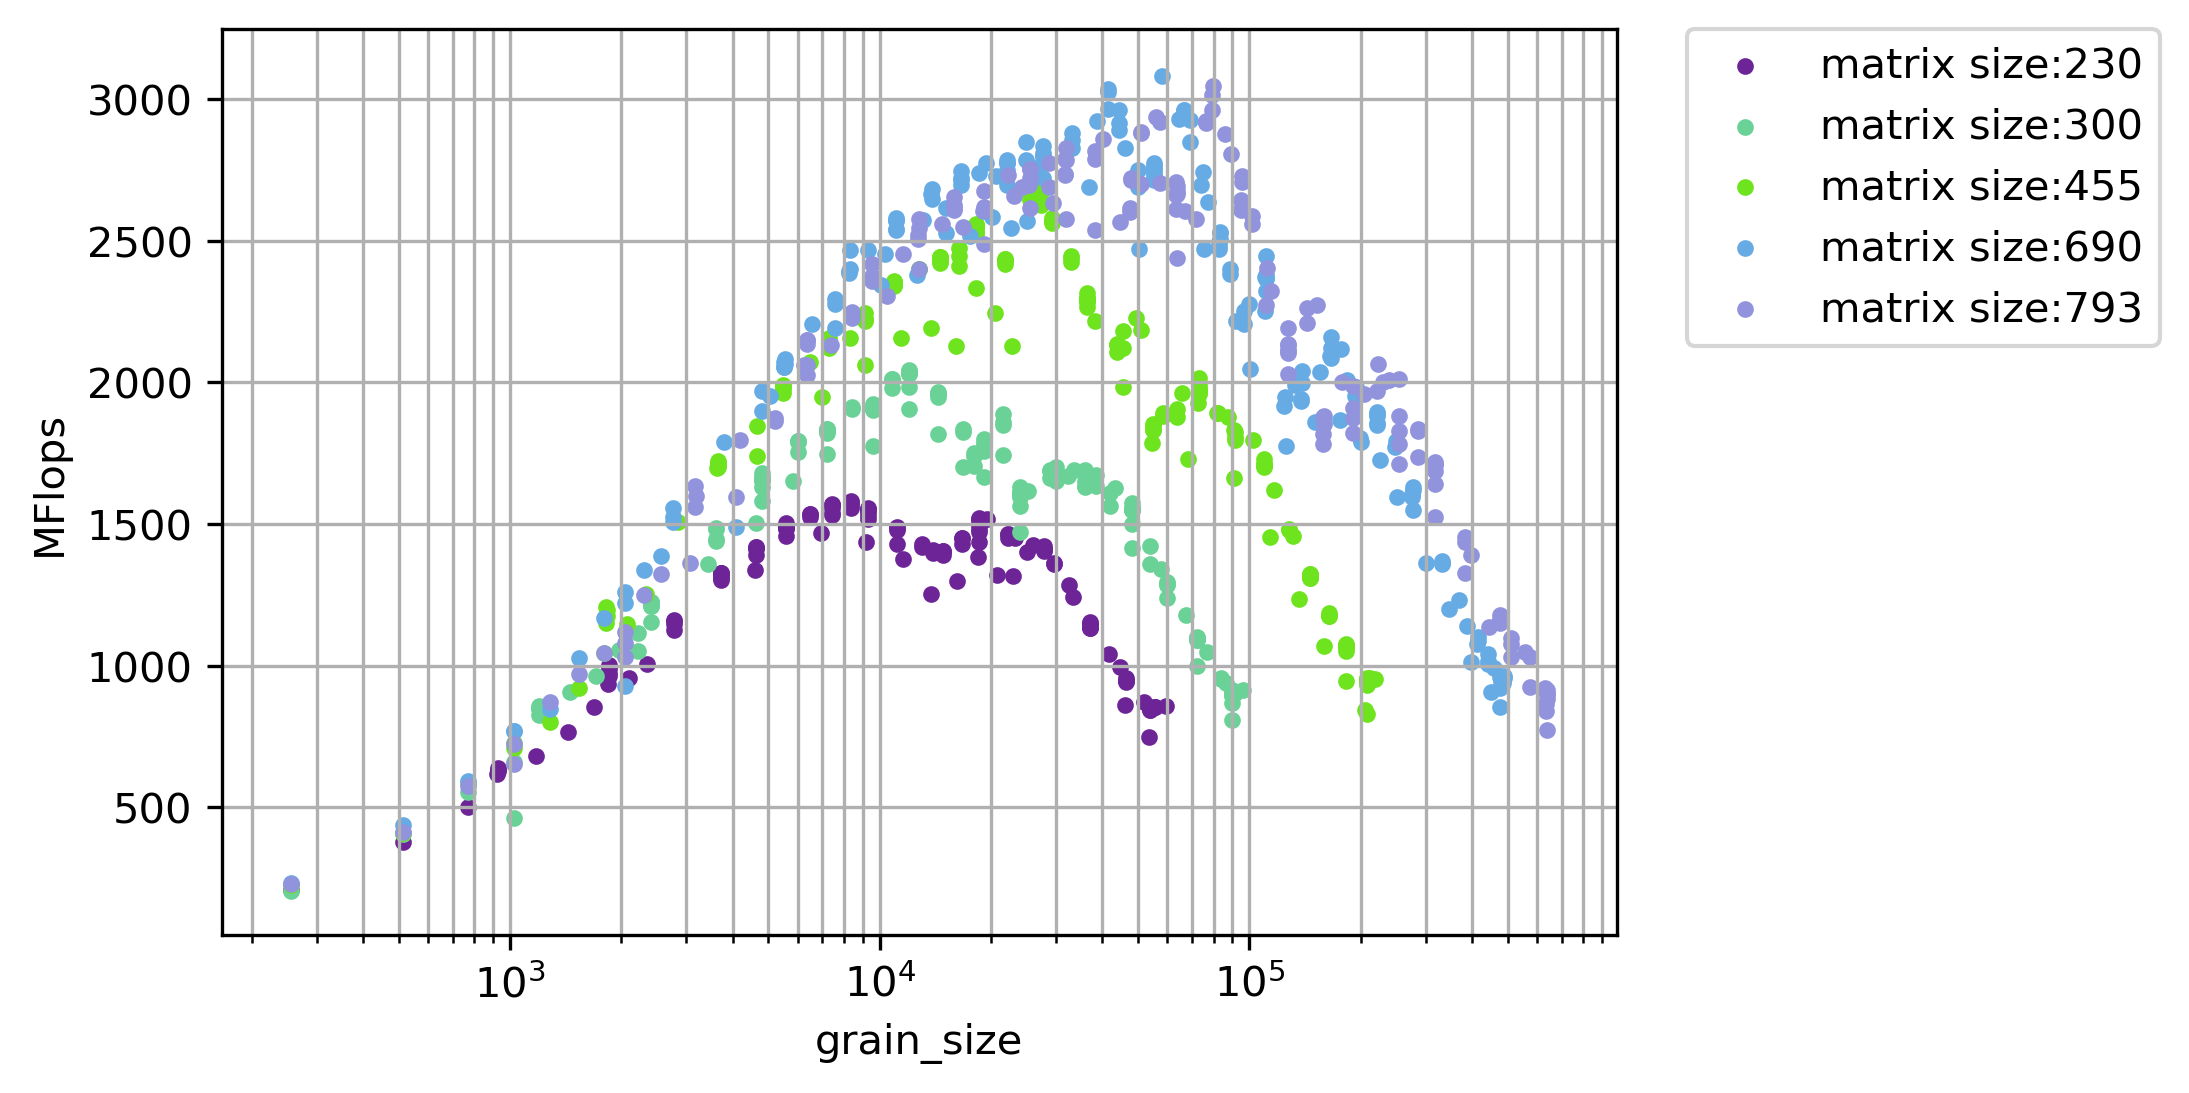
\includegraphics[scale=.75]{images/fig8.png}
	\caption{The results obtained from running $DMATDMATADD$ benchmark through Blazemark for 5 different matrix sizes on $4$ cores}	
	\label{fig7}
\end{figure}

\begin{figure}[H]
	\subfloat[]
	{\centering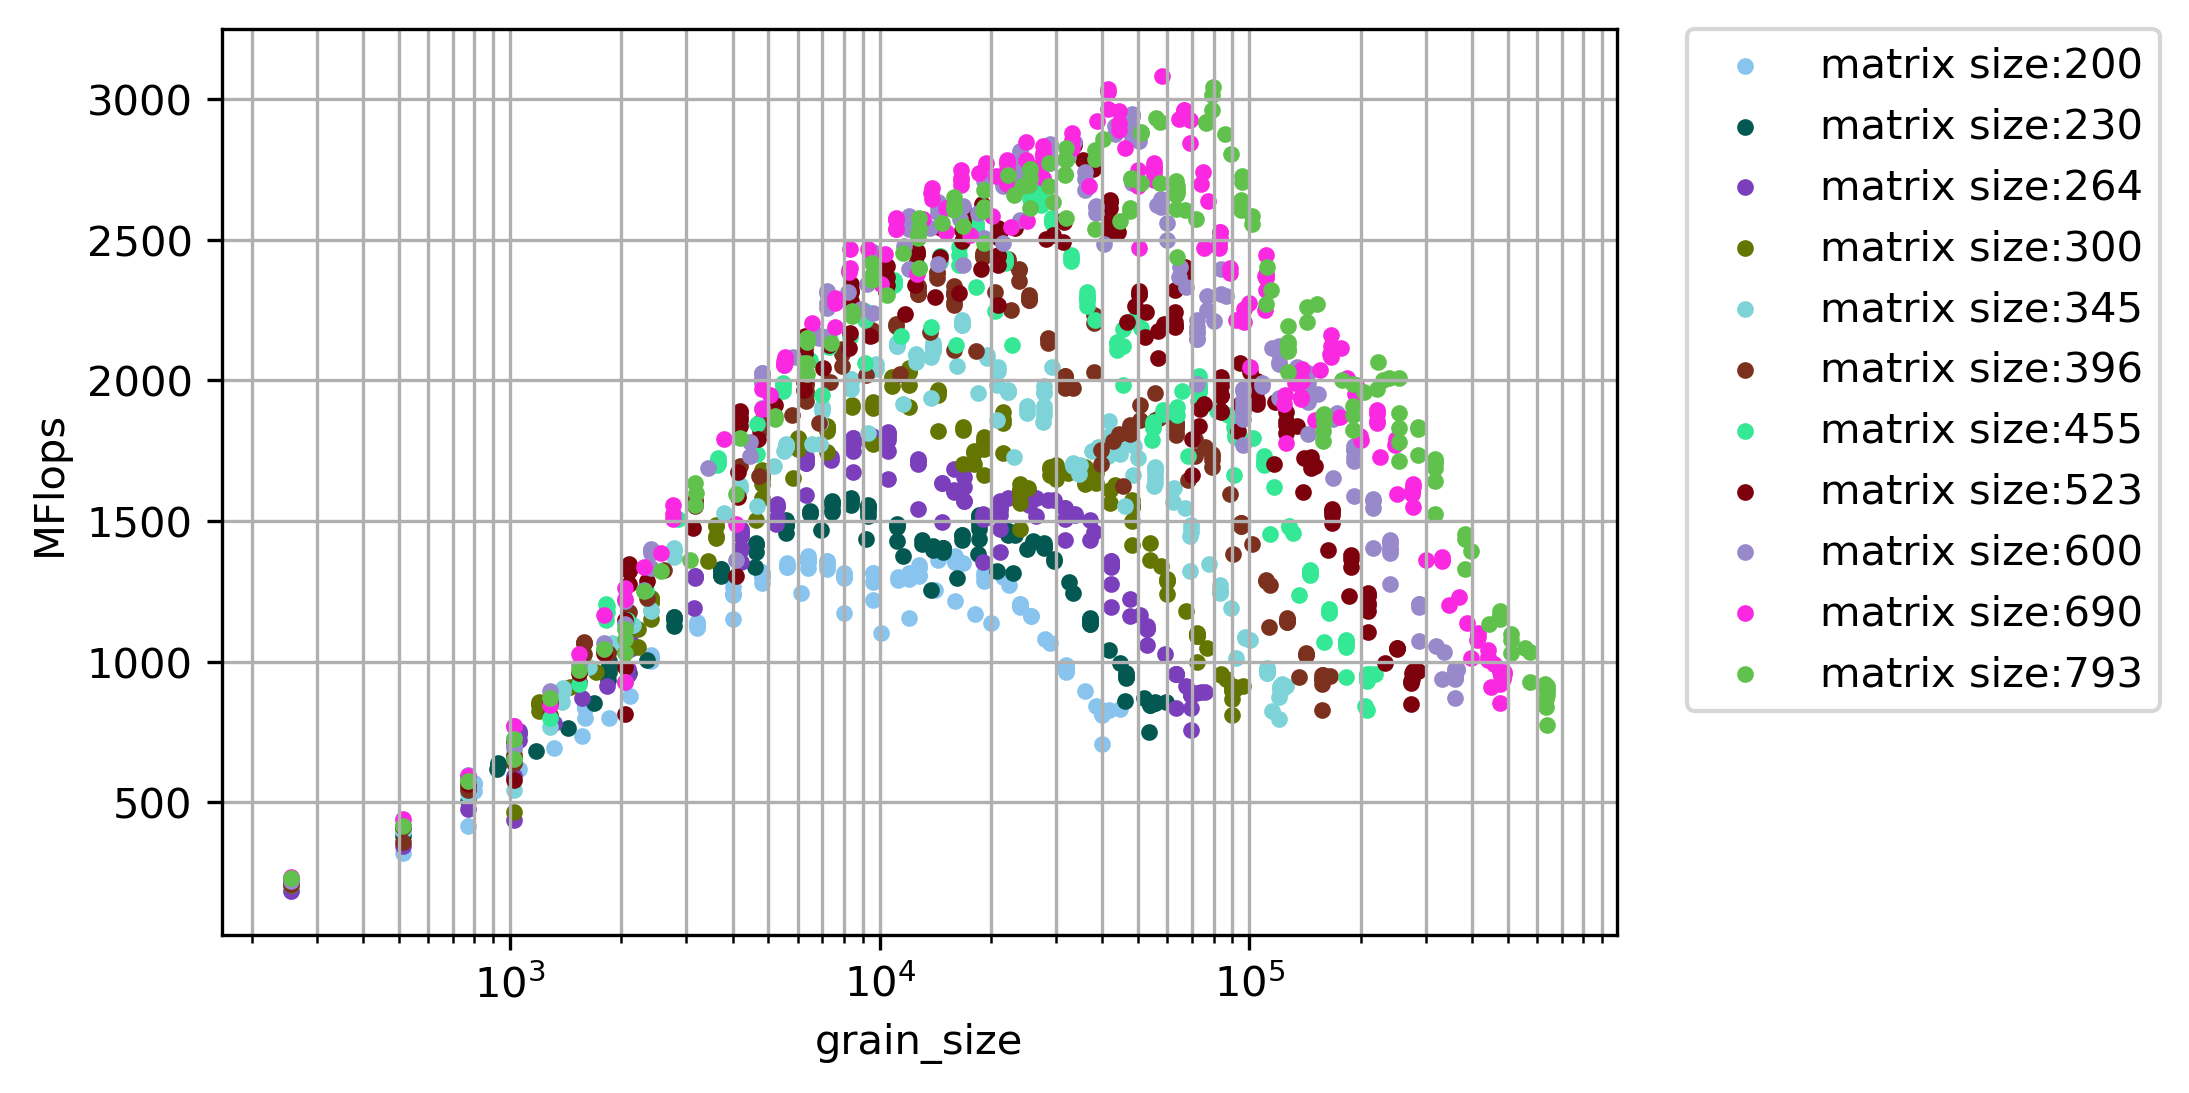
\includegraphics[scale=.75]{images/fig11.png}	
	\label{fig8:a}}

	\subfloat[]{
	\centering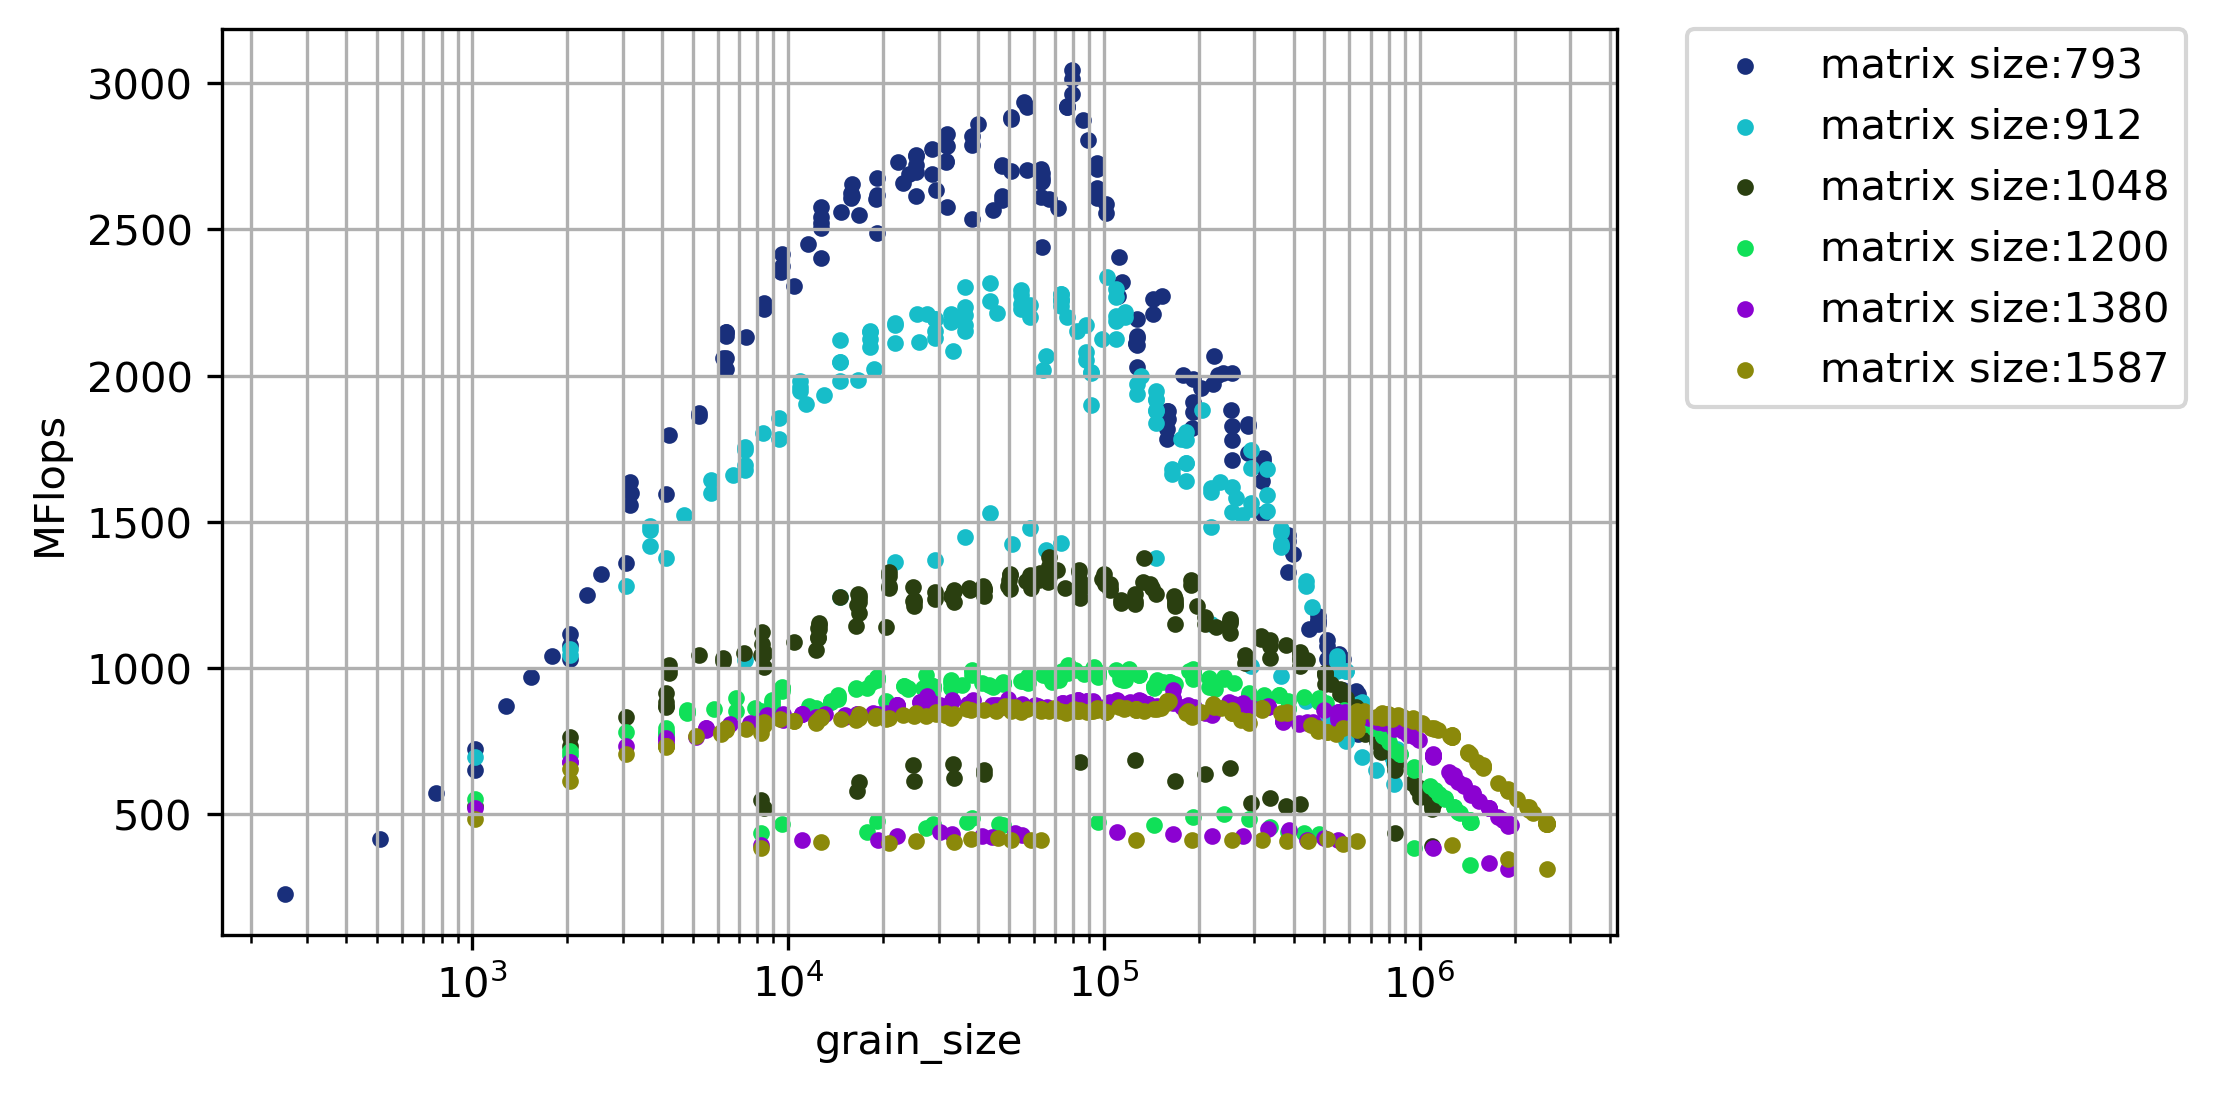
\includegraphics[scale=.75]{images/fig12.png}
	\label{fig8:b}}
	\caption{Throughput vs. grain size graph obtained from running $DMATDMATADD$ benchmark  on $4$ cores for matrix sizes (a) smaller than 912$\times$912 and (b) larger than 912$\times$912}
	\label{fig8}	
\end{figure}

\begin{figure}[H]
	\centering
	\hspace*{-2cm}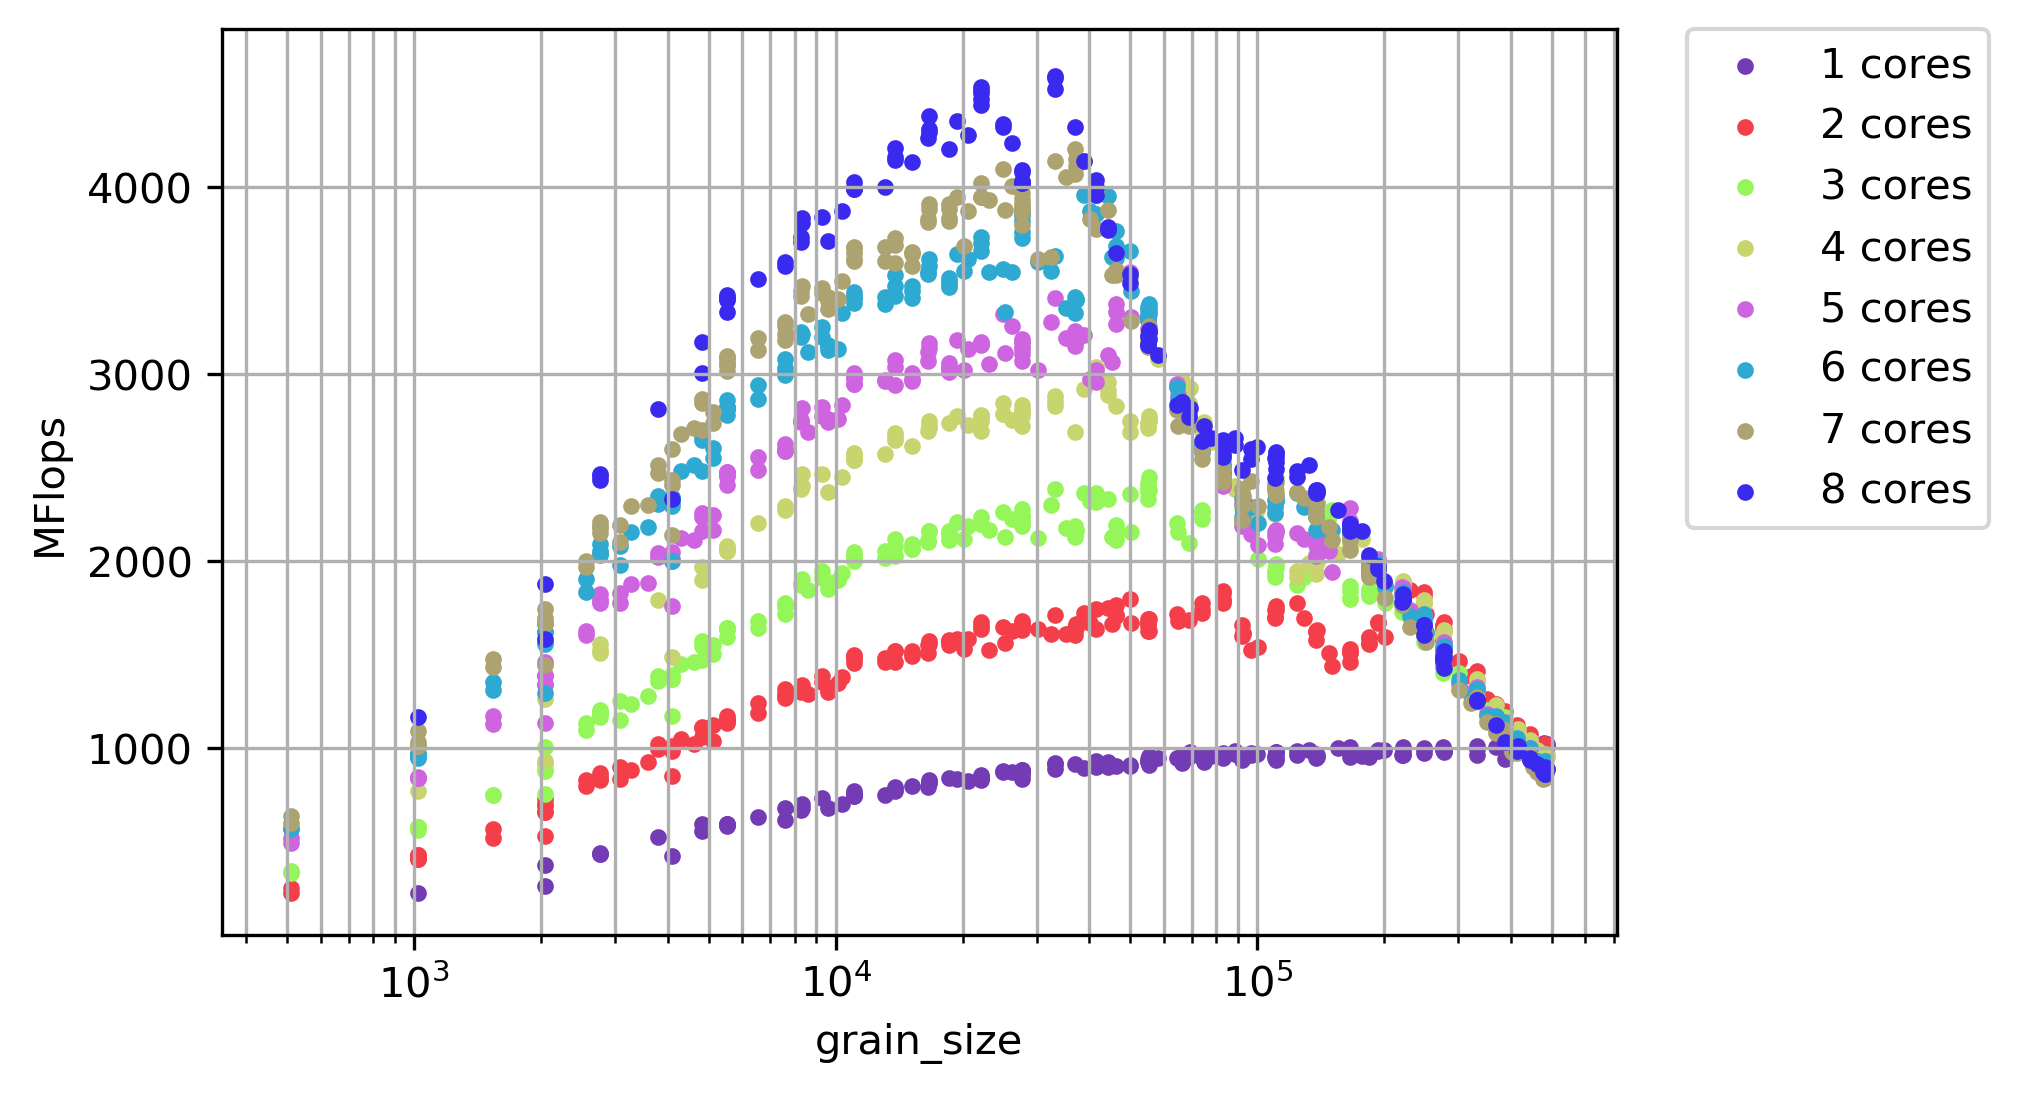
\includegraphics[scale=.75]{images/fig13.png}
	\caption{The results obtained from running $DMATDMATADD$ benchmark through Blazemark for matrix size 690$\times$690 on different number of cores}	
	\label{fig9}
\end{figure}


%\begin{figure}[H]
%	\centering
%	\hspace*{-2cm}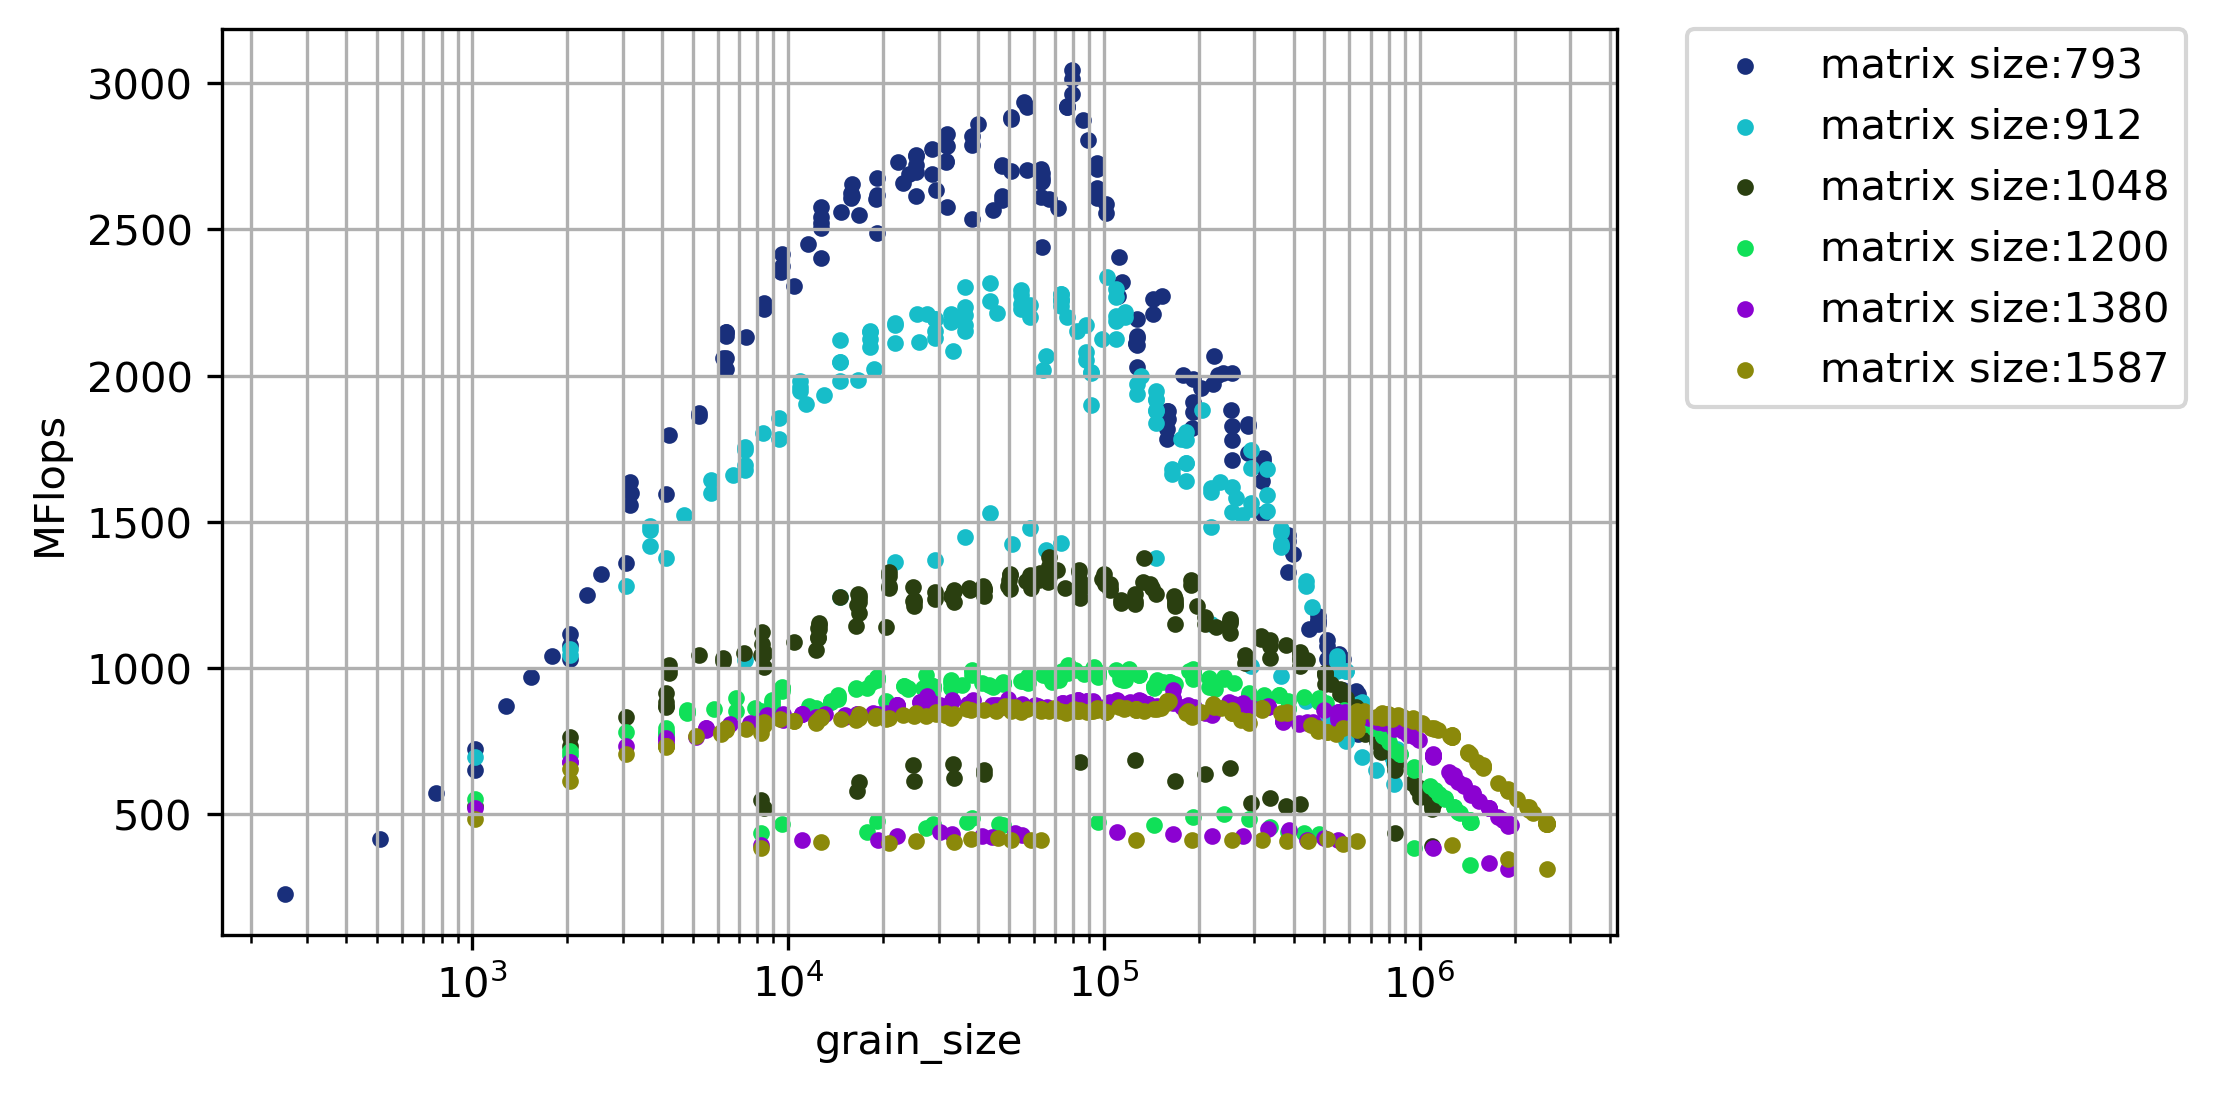
\includegraphics[scale=.75]{images/fig12.png}
%	\caption{The results obtained from running $DMATDMATADD$ benchmark through Blazemark for 5 different matrix sizes on $4$ cores}	
%	\label{fig9}
%\end{figure}